%adapted from https://tikz.net/neural_networks/
\documentclass[border=3pt,tikz]{standalone}
\usepackage{amsmath} % for aligned
%\usepackage{amssymb} % for \mathbb
\usepackage{tikz}
%\usepackage{etoolbox} % for \ifthen
\usepackage{listofitems} % for \readlist to create arrays
\usetikzlibrary{arrows.meta} % for arrow size
\usepackage[outline]{contour} % glow around text
\usepackage[sfdefault]{carlito}
\contourlength{1.4pt}

\tikzset{>=latex} % for LaTeX arrow head
\usepackage{xcolor}
\colorlet{myred}{red!80!black}
%\colorlet{myblue}{blue!80!black}
\colorlet{myblue}{black!50}
\colorlet{mygreen}{green!60!black}
\colorlet{myorange}{orange!70!red!60!black}
\colorlet{mydarkred}{red!30!black}
%\colorlet{mydarkblue}{blue!40!black}
\colorlet{mydarkblue}{black!70}
\colorlet{mydarkgreen}{green!30!black}
\tikzstyle{node}=[thick,circle,draw=myblue,minimum size=22,inner sep=0.5,outer sep=0.6]
\tikzstyle{node in}=[node,green!20!black,draw=mygreen!30!black,fill=mygreen!25]
\tikzstyle{node hidden}=[node,blue!20!black,draw=myblue!30!black,fill=myblue!20]
\tikzstyle{node convol}=[node,orange!20!black,draw=myorange!30!black,fill=myorange!20]
\tikzstyle{node out}=[node,red!20!black,draw=myred!30!black,fill=myred!20]
\tikzstyle{connect}=[thick,mydarkblue] %,line cap=round
\tikzstyle{connect arrow}=[-{Latex[length=4,width=3.5]},thick,mydarkblue,shorten <=0.5,shorten >=1]
\tikzset{ % node styles, numbered for easy mapping with \nstyle
  node 1/.style={node in},
  node 2/.style={node hidden},
  node 3/.style={node out},
}
\def\nstyle{int(\lay<\Nnodlen?min(2,\lay):3)} % map layer number onto 1, 2, or 3

\begin{document}

% NEURAL NETWORK with coefficients, no arrows
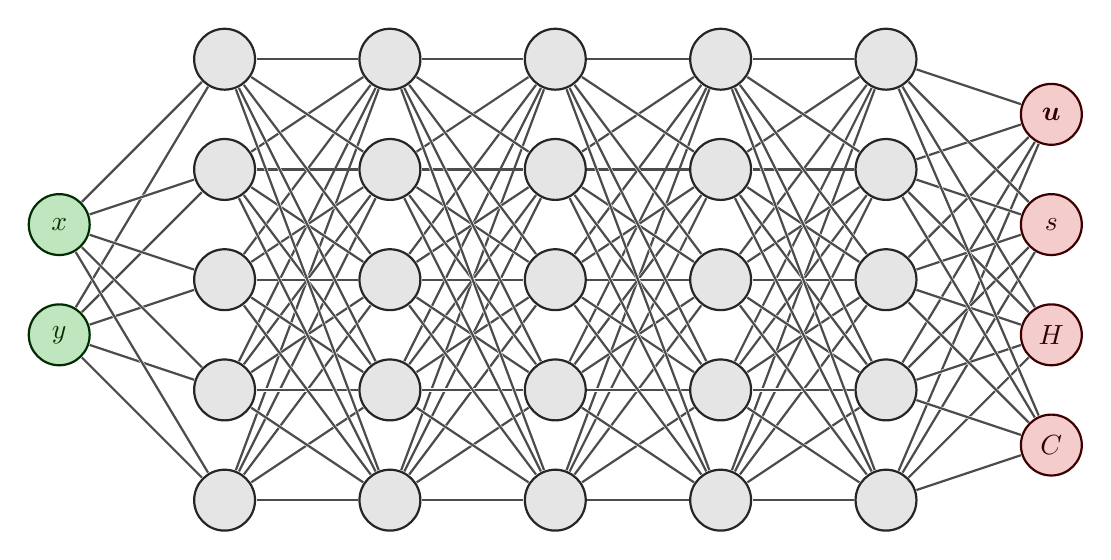
\begin{tikzpicture}[x=2.1cm,y=1.4cm]
  %\message{^^JNeural network without arrows}
  \readlist\Nnod{2,5,5,5,5,5,4} % array of number of nodes per layer
  
  \message{^^J  Layer}
  \foreachitem \N \in \Nnod{ % loop over layers
    \def\lay{\Ncnt} % alias of index of current layer
    \pgfmathsetmacro\prev{int(\Ncnt-1)} % number of previous layer
    \message{\lay,}
    \foreach \i [evaluate={\y=\N/2-\i; \x=\lay; \n=\nstyle;}] in {1,...,\N}{ % loop over nodes
      
      % NODES

      
      \ifnum \lay=1 %First layer
        \ifnum \i=1
        \node[node \n] (N\lay-\i) at (\x,\y) {$x$};
        \else \ifnum \i=2
        \node[node \n] (N\lay-\i) at (\x,\y) {$y$};
        \fi \fi
      \else \ifnum \lay=\Nnodlen %Last layer
        \ifnum \i=1
        \node[node \n] (N\lay-\i) at (\x,\y) {${\boldsymbol{u}}$};
        \else \ifnum \i=2
        \node[node \n] (N\lay-\i) at (\x,\y) {$s$};
        \else \ifnum \i=3
        \node[node \n] (N\lay-\i) at (\x,\y) {$H$};
        \else \ifnum \i=4
        \node[node \n] (N\lay-\i) at (\x,\y) {$C$};
        \fi \fi \fi \fi
      \else %hidden layer
        %\node[node \n] (N\lay-\i) at (\x,\y) {$a_\i^{(\prev)}$};
        \node[node \n] (N\lay-\i) at (\x,\y) {};
      \fi \fi
      
      % CONNECTIONS
      \ifnum\lay>1 % connect to previous layer
        \foreach \j in {1,...,\Nnod[\prev]}{ % loop over nodes in previous layer
          \draw[connect,white,line width=1.2] (N\prev-\j) -- (N\lay-\i);
          \draw[connect] (N\prev-\j) -- (N\lay-\i);
          %\draw[connect] (N\prev-\j.0) -- (N\lay-\i.180); % connect to left
        }
      \fi % else: nothing to connect first layer
      
    }
  }
  
  % LABELS
  %\node[above=5,align=center,mygreen!60!black] at (N1-1.90) {Input\\[-0.2em]layer};
  %\node[above=4,align=center,myblue!60!black] at (N4-1.90) {Hidden layers};
  %\node[above=8,align=center,myred!60!black] at (N\Nnodlen-1.90) {Output\\[-0.2em]layer};

\end{tikzpicture}

\end{document}